\begin{figure}
    \begin{center}
    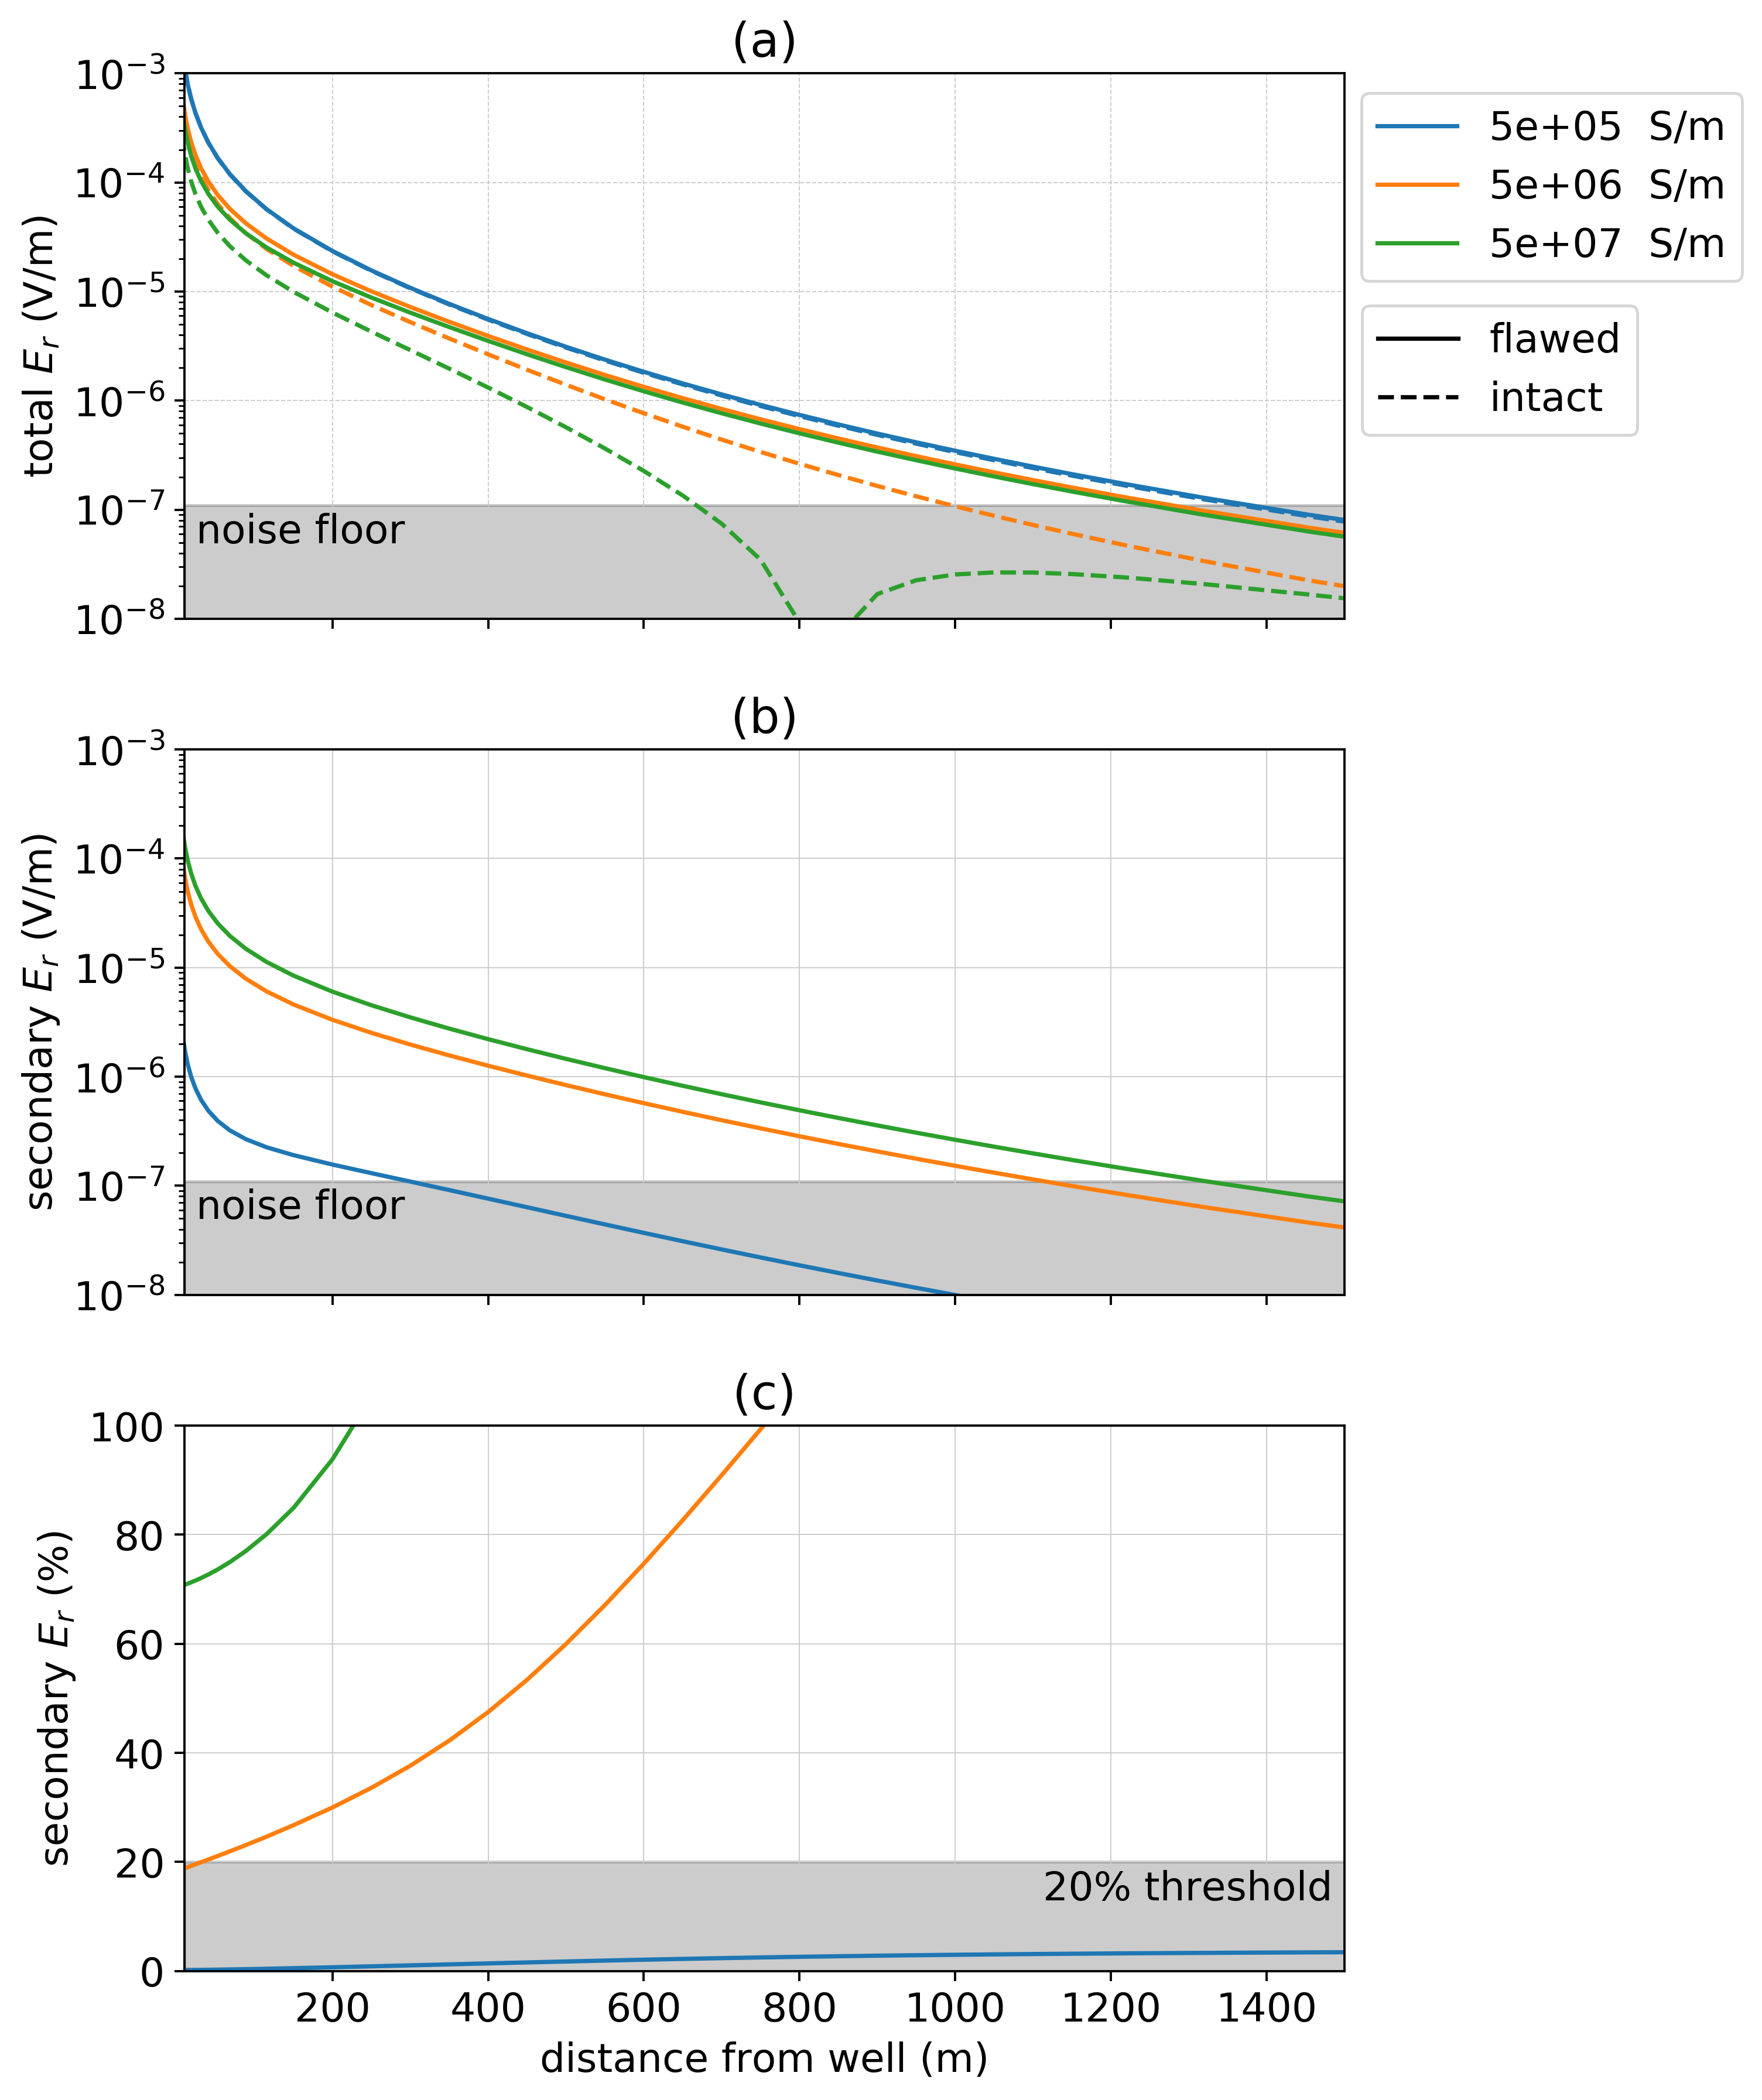
\includegraphics[width=0.8\textwidth]{figures/dc_casing/integrity_conductivity_casing.png}
    \end{center}
\caption{
    Radial electric field as the conductivity of the casing is varied for a 1 km well with a 10 m flaw at 500 m depth.
    The positive electrode is connected to the top of the casing, the negative electrode
    is positioned 500 m away and data are measured along a line $90^\circ$ from the
    source electrodes. In (a), we show the total electric field for three different casing conductivities,
    each indicated on the legend. The solid lines indicate the response of the flawed well and the dashed lines indicate the response of the intact well (the primary).
    In (b), the secondary radial electric field is plotted and in (c), we show the
    secondary radial electric field as a percentage of the primary.
}
\label{fig:integrity_conductivity_casing}
\end{figure}
